\documentclass[main.tex]{subfiles}


\begin{document}
	\section{Introduction}
	In this thesis we look at phenomena arising from the discrete translational symmetry of crystals. As a first example we look at the nearly free electron model in one dimension. This model illustrates some key concepts which will be useful later on, like reciprocal lattice vectors and how the dispersion relation change with the potential strength.
	
	\subsection{Nearly Free Electron model in One Dimension}\label{sec:nearly_free}
	The nearly free electron model is, as the name suggests, a model in which electrons are moving in a medium with a small perturbing potential, such that they are nearly free. As such we assume that electrons are essentially free, but experience some small periodic potential that we treat as a perturbation.
	
	In general, the Hamiltonian is
	\begin{equation}
		H = H_0 + H', \quad H_0 = \frac{p^2}{2m}, \quad H' = V(x) = V(x + na), n \in \mathbb{Z}
	\end{equation}
	where $ a $ is the spacing between atoms. In this case we are dealing with plane waves (at least to zeroth order in perturbation theory) $ \ket{k} $, with zeroth order energies $ E_0(k)= \hbar^2 k^2/2m $. Now, to calculate anything in perturbation theory, we need the matrix elements of the potential $ \braket{k' | V | k} $. These are
	\begin{equation}
		\braket{k' | V | k} = \infint e^{-i(k'-k)x} V(x) \equiv V_{k'-k}.\ud x
	\end{equation}
	Due to the periodicity of the potential we can write this integral as a sum of integrals by setting $ x=x'+na $
	\begin{equation}
		\braket{k' | V | k} = \sum_{n = -\infty}^{\infty} e^{-i(k'-k) na} \int_{0}^{a} e^{-i(k'-k)x'} V(x').\ud x'
	\end{equation}
	This sum is infinite for a discrete set of values $ k'-k $, namely
	\begin{equation}
		k'-k = \frac{2\pi j}{a} \equiv G_j, \quad j \in \mathbb{Z}
	\end{equation}
	where $ G_j $ is called a reciprocal lattice vector (with $ x_n=na $ being a direct lattice vector). If $ k'-k $ is not a reciprocal lattice vector, then this sum is just 0, akin to how roots of unity sum to 0.(\textbf{REF FOR THIS?})
	
	Due to this, there is only a discrete set of values in $ k $-space that contribute to the energy (and wave function) of $ \ket{k} $, meaning that $ \ket{k} $ can only scatter into another state if it is separated by a reciprocal lattice vector. Further interesting things happen if the energies of some other plane waves are equal to that of $ \ket{k} $. Due to the parabolic dispersion of the plane waves, the first case where these conditions apply is for $ k $ around $ \pi/a $ and $ k'=k + G_{-1} \approx -\pi/a $. Here $ E_0(k) = E_0(k') $, and we are at a reciprocal lattice vector (the smallest non-trivial one, in fact). Due to this we need to treat the problem in degenerate perturbation theory.
	
	For this case, there are 4 relevant matrix elements:
	\begin{align}
		\braket{k|H|k} = E_0(k) + V_0, \quad \braket{k'|H|k'} = E_0(k+G_{-1}) + V_0, \quad \braket{k'|H|k} = \braket{k|H|k'}^* = V_G.
	\end{align}
	For simplicity we assume $ V_0 = 0 $, as it is just a constant. Around these values of $ k $ and $ k' $ we take the wave function as $ \ket{\psi} = \alpha \ket{k} + \beta \ket{k+G_{-1}} $, which means that the energy can be found as the eigenvalue to the Hamiltonian in this "two-dimensional" subspace of these two plane waves:
	\begin{equation}
		\begin{pmatrix}
			E_0(k) & V_G^* \\ V_G & E_0(k+G_{-1})
		\end{pmatrix} \begin{pmatrix}
		\alpha \\ \beta
		\end{pmatrix} = E \begin{pmatrix}
		\alpha \\ \beta
		\end{pmatrix}, \quad \Rightarrow \quad (E_0(k)-E)(E_0(k+G_{-1})-E) - |V_G|^2 = 0.
	\end{equation}
	In the simple case of $ k $ being exactly $ \pi/a $, the energy is just $ E_{\pm} = E_0(k) \pm | V_G| $, which means there is a band gap of $ 2|V_G| $ at $ \pm \pi/a $. In the not-so-simple case of $ k = \pi/a - \delta $, where $ \delta $ is some small (positive) number, we get
	\begin{equation}
		E_0(k) = \frac{\hbar^2}{2m}\bb{\pp{\frac{\pi}{a}}^2 + \delta^2 - \frac{2\pi}{a}}, \quad E_0(k+G_{-1}) = \frac{\hbar^2}{2m} \bb{\pp{\frac{\pi}{a}}^2 + \delta^2 + \frac{2\pi}{a}},
	\end{equation}
	\begin{wrapfigure}{r}{2in}
		\begin{center}
			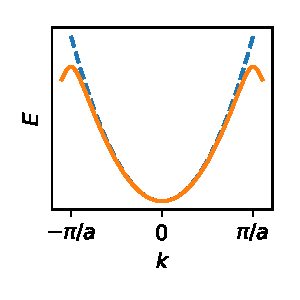
\includegraphics[width=\linewidth]{figures/nearly_free.pdf}
		\end{center}
		\caption{Dispersion relation of electrons in the (nearly) free electron model, for $ -\pi/a \leq k \leq \pi/a $. The solid orange line is for a nearly free electron, whilst the dashed blue line is for a free electron.}
		\label{fig:nearly_free}
	\end{wrapfigure}
	with an eigenenergy of
	\begin{equation}
		E_{\pm} = \frac{\hbar^2}{2m} \bb{\pp{\frac{\pi}{a}}^2 + \delta^2 } \pm |V_G| \sqrt{1+ \pp{\frac{2\pi\hbar^2 \delta}{2m a |V_G|}}^2 }.
	\end{equation}
	As we are dealing with $ \delta \approx 0 $, we expand the square root to second order and get
	\begin{equation}
		E_{\pm} = \frac{\hbar^2 \pi^2}{2m a^2} \pm |V_G| + \frac{\hbar^2 \delta^2}{2m} \bb{1 \pm \frac{\hbar^2 \pi^2}{m a^2 |V_G|}}
	\end{equation}
	where the second term in brackets is larger than unity (for small perturbations) \cite{simon}, such that the dispersion is a negative parabola in $ \delta $, for $ E_- $. This all means that for $ k =\pi/a$ (or equivalently $ -\pi/a $), a gap appears in the dispersion relation, and the energy in the lower branch is lowered, such that $ \partial E/ \partial k =0$ (see figure \ref{fig:nearly_free}). As it turns out this is happens for any reciprocal lattice vector, with $ k = j \pi/a $ and $ k'=-j \pi /a = k+G_{-j}$. These characteristics (scattering only being allowed for states separated by reciprocal lattice vectors, and bands of energy appearing at regular intervals) also appear in systems of higher dimensions, as we will see in sections \ref{sec:scattering} and \ref{sec:band_structure}.
	
	
	
	\subsection{Bloch's Theorem}
	In the previous section we considered the case of an electron in a weak periodic potential, where the wave function is essentially a plane wave. But this always the for real materials? Can we really be sure that we can treat the wave function as plane waves even when the potential strength is cranked up? It turns out we can, and the proof of that lies with Bloch's theorem.
	
	The assumption here is that we are working with a periodic potential, such that $ V(\V{r} + \V{R}) $ for all lattice points. As such the full Hamiltonian has a discrete translational symmetry, which means that all translation operators $ \hat{T}_{\V{R}} $ (that translate by any lattice vector $ \V{R} $) commute with the Hamiltonian: $ [\hat{H}, \hat{T}_{\V{R}}] = 0$. This further means that we can simultaneously diagonalize these operators and find a shared basis of eigenstates.
	
	The eigenvalue of the translation operator must have a magnitude of unity, as it otherwise would break the translation symmetry inherent to the system. So the only possible eigenvalue is a phase shift. Further we need all translation operators to commute with each other, and $ \hat{T}_{\V{R}_1} \hat{T}_{\V{R}_2} = \hat{T}_{\V{R}_1 + \V{R}_2} $. With these restrictions the only possible eigenvalue is
	\begin{equation}
		\hat{T}_{\V{R}} \psi(\V{r}) = e^{i\V{k} \D\V{R}} \psi(\V{r}) = \psi(\V{r}+\V{R}),
	\end{equation}
	where the last equality is just the definition of the translation operator. This means we can write the wave function as a plane wave times some function that has the same periodicity as the crystal:
	\begin{equation}
		\psi(\V{r}) = e^{i\V{k} \D \V{r}} u(\V{r}),
	\end{equation}
	where $ u(\V{r}) $ carries this periodicity of the crystal. As we shall see in section \ref{sec:band_structure}, we can write a periodic function as a sum of plane waves over reciprocal lattice vectors. This then also applies to $ u $, as it is periodic in the unit cell. Due to this, we can write the wave function as
	\begin{equation}\label{key}
		\psi(\V{r}) = \sum_{\V{G}} u_{\V{G},\V{k}} e^{i(\V{G} + \V{k}) \D \V{r}},
	\end{equation}
	where $ u_{\V{G},\V{k}} $ is some number. This will be important in the context of scattering and band structure as we will see in sections \ref{sec:scattering} and \ref{sec:band_structure}.
	
	
	
	
	\subsection{General implementation}
	All of the programs in this project will be implemented in the open source programming language \href{www.python.org}{Python}, using the standard library, along with the \href{www.numpy.org}{NumPy} and \href{www.matplotlib.org}{Matplotlib} packages. Numpy adds the necessary tools for handling arrays and linear algebra operations, whilst Matplotlib is used for plotting the results.
	
	One thing to note is that doing numerical calculations will lead to some numerical error. As such testing for numerical equality will often time yield the "wrong" result. Because of this, we employ the \texttt{isclose} function provided by NumPy, which takes 4 arguments: \texttt{a}, \texttt{b}, \texttt{atol} and \texttt{rtol}. \texttt{a} and \texttt{b} are the numerical values to be tested for equality, \texttt{atol} is the absolute tolerance and \texttt{rtol} is the relative tolerance. The function then tests if $|\texttt{a}-\texttt{b}| \leq (\texttt{atol}+ \texttt{rtol} \D |\texttt{b}|)$, with default values for \texttt{atol} and \texttt{rtol} being $ 1 \D 10^{-8} $ and $ 1 \D 10^{-5} $ respectively.
	
	
	
\end{document}